\graphicspath{{./img/}}

\section*{\LARGE{Введение}}
\addcontentsline{toc}{section}{Введение}
\textbf{Цель:} Создать чат-бота "<очередь"> для соц. сети Telegram.

\textbf{Задачи:}
\begin{itemize}
	\item Создать контейнер Docker для проекта;
	\item Запустить приложение на сервере.
\end{itemize}

\clearpage

\section*{\LARGE{Выполнение итогового проекта}}
\addcontentsline{toc}{section}{Выполнение итогового проекта}

\section{Dockerfile}
Контейнер Docker --- это образ Docker, вызванный к жизни.
Это --- самодостаточная операционная система, в которой имеется только самое
необходимое и код приложения. Образы Docker являются результатом процесса
их сборки, а контейнеры Docker --- это выполняющиеся образы.\par
В самом сердце Docker находятся файлы Dockerfile.
Подобные файлы сообщают Docker о том, как собирать образы, на основе
которых создаются контейнеры. Контейнер бота и базы данных представлен
в листингах ниже.

\begin{lstlisting}[language=Dockerfile
	, caption=\leftline{Dockerfile бота}
	, label=lst:DF:bot
	, columns=flexible
	]
FROM python:latest
WORKDIR /bot
RUN pip install --upgrade pip
ADD requirements.txt requirements.txt
RUN pip install -r requirements.txt
COPY . /bot
CMD ["python", "-u", "main.py"]
\end{lstlisting}

Тут импортируется образ python контейнера, устанавливается requirements
и запускается main.py.

\begin{lstlisting}[language=Dockerfile
	, caption=\leftline{Dockerfile базы данных}
	, label=lst:DF:db
	, columns=flexible
	]
FROM postgres:latest
ENV POSTGRES_PASSWORD=postgres
ENV POSTGRES_USER=postgres
ENV POSTGRES_DB=queue
\end{lstlisting}

Тут импортируется образ postgres контейнера, с необходдтимыми параметрами
базы данных.


\section{Docker Compose}
Docker применяется для управления отдельными контейнерами (сервисами),
из которых состоит приложение. Docker Compose используется для одновременного
управления несколькими контейнерами, входящими в состав приложения.
Этот инструмент предлагает те же возможности, что и Docker,
но позволяет работать с более сложными приложениями.
Ниже представлен листинг Docker Compose проекта.

\begin{lstlisting}[language=Dockerfile
	, caption=\leftline{Dockerfile базы данных}
	, label=lst:DС
	, columns=flexible
	]
version: "3.9"
services:
  bot:
    build:
      context: './bot/'
      dockerfile: "./Dockerfile"
    restart: always
  postgres:
    image: postgres:13.3
    environment:
      POSTGRES_DB: "queue"
      POSTGRES_USER: "postgres"
      POSTGRES_PASSWORD: "postgres"
    build:
      context: './database'
      dockerfile: "./Dockerfile"
    ports:
      - "5432:5432"
\end{lstlisting}

Тут запускаються два контейнера bot для бота, postgres для базы данных
где выставляеться порт базы данных.

\section{Развертывание контейнера на сервере}
Docker Compose был развернут на собственном сервере с помощью трех команд:

\begin{verbatim}
git pull
docker-compose build
docker-compose up
\end{verbatim}

\begin{figure}[h!tp]
  \centering
  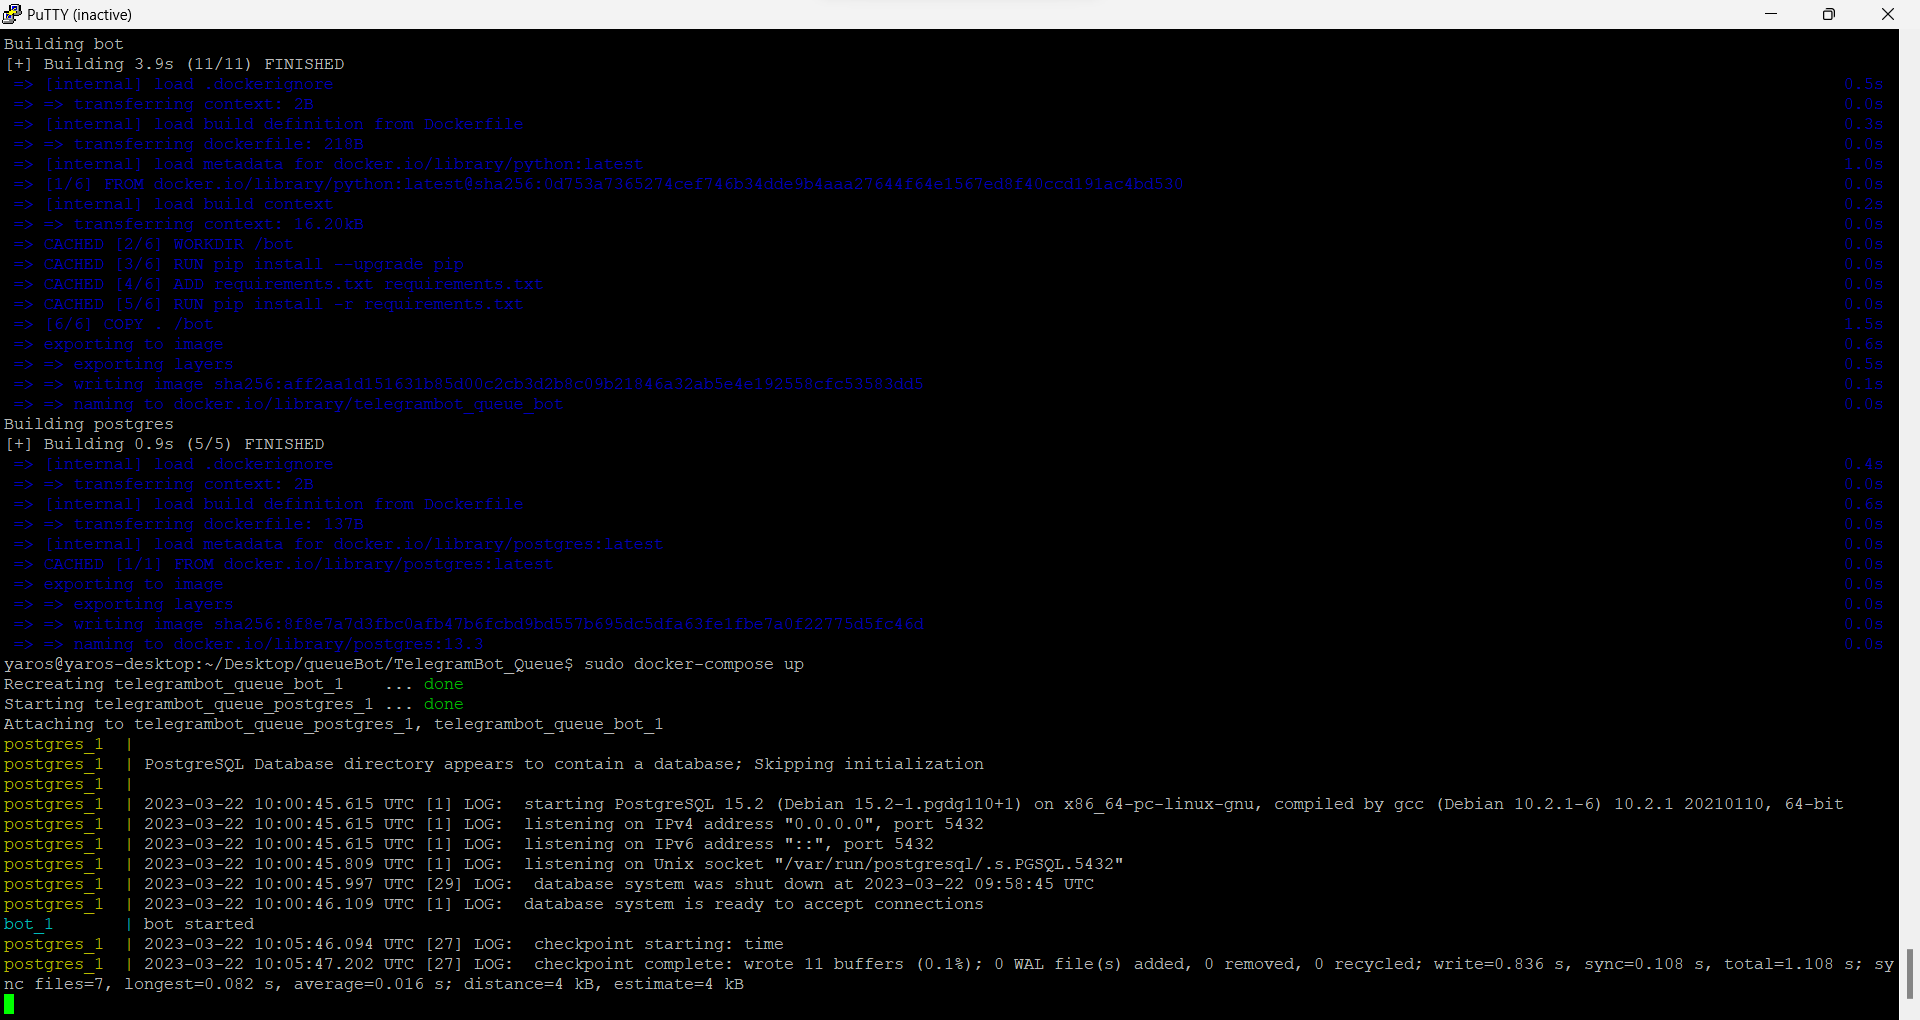
\includegraphics[width=1\textwidth]{server_run}
  \caption{Развертывание контейнера на сервере}
  \label{fig:server:run}
\end{figure}

